\chapter{Vygotskian Autotelic Agents}
\label{chap:foundation_vaai}

\section{From Autotelic to Vygotkian Agents}

\begin{abstract} % 214 mots
Building autonomous agents able to grow open-ended repertoires of skills across their lives is a fundamental goal of artificial intelligence (\ai). A promising developmental approach recommends the design of intrinsically motivated agents that learn new skills by generating and pursuing their own goals\,---\,\textit{autotelic agents}. But despite recent progress, existing algorithms still show serious limitations in terms of goal diversity, exploration, generalization or skill composition. 
% 
This perspective calls for the immersion of autotelic agents into \textit{rich socio-cultural worlds}, an immensely important attribute of our environment that shapes human cognition but is mostly omitted in modern \ai. 
Inspired by the seminal work of Vygotsky, we propose \textit{Vygotskian autotelic agents}\,---\,agents able to internalize their interactions with others and turn them into \textit{cognitive tools}. We focus on language and show how its structure and informational content may support the development of new cognitive functions in artificial agents like it does in humans.
% 
We justify the approach by uncovering several examples of new artificial cognitive functions emerging from interactions between language and embodiment in recent works at the intersection of deep reinforcement learning and natural language processing. Looking forward, we highlight future opportunities and challenges for a Vygotskian Autotelic AI research, including the use of language models as cultural models supporting artificial cognitive development. 

\end{abstract}

\subsection*{Introduction}
%our goal
Humans are remarkable examples of lifelong open-ended learners. They learn to recognize objects and crawl as infants, learn to ask questions and interact with peers as toddlers, learn to master engineering, science, or arts as adults. A fundamental goal of artificial intelligence (\ai) is to build autonomous agents capable of growing such open-ended repertoires of skills. 

% RL and deep RL
\textit{Reinforcement learning} (\rl) offers a mathematical framework to formalize and tackle skill learning problems. For an embodied and situated \rl agent, \textit{learning a skill} (\eg playing chess) is about learning to act so as to maximize future \textit{rewards} measuring progression in that skill (\eg +1 for winning a game, -1 for losing it).\cite{sutton_introduction_1998} Extensions based on modern deep learning methods (deep \rl) have recently made the headlines by solving a wealth of problems we thought only humans could solve: beating chess and go world champions,\cite{silver2016mastering} controlling stratospheric balloons,\cite{bellemare2020autonomous} or even maintaining plasma in fusion reactors.\cite{degrave2022magnetic} But human chess world champions can also run, cook, draw a cat, or make a friend laugh. Humans are proficient in a wide diversity of tasks, most of which they just invent for themselves. The \rl framework, in its standard form, considers a single predefined reward function and, thus, must be extended (see Figure~\ref{fig:rl_arl_varl}, a).

\vspace{.4cm}

\begin{figure}[!ht]
    \centering
    \captionsetup{width=.85\linewidth}
    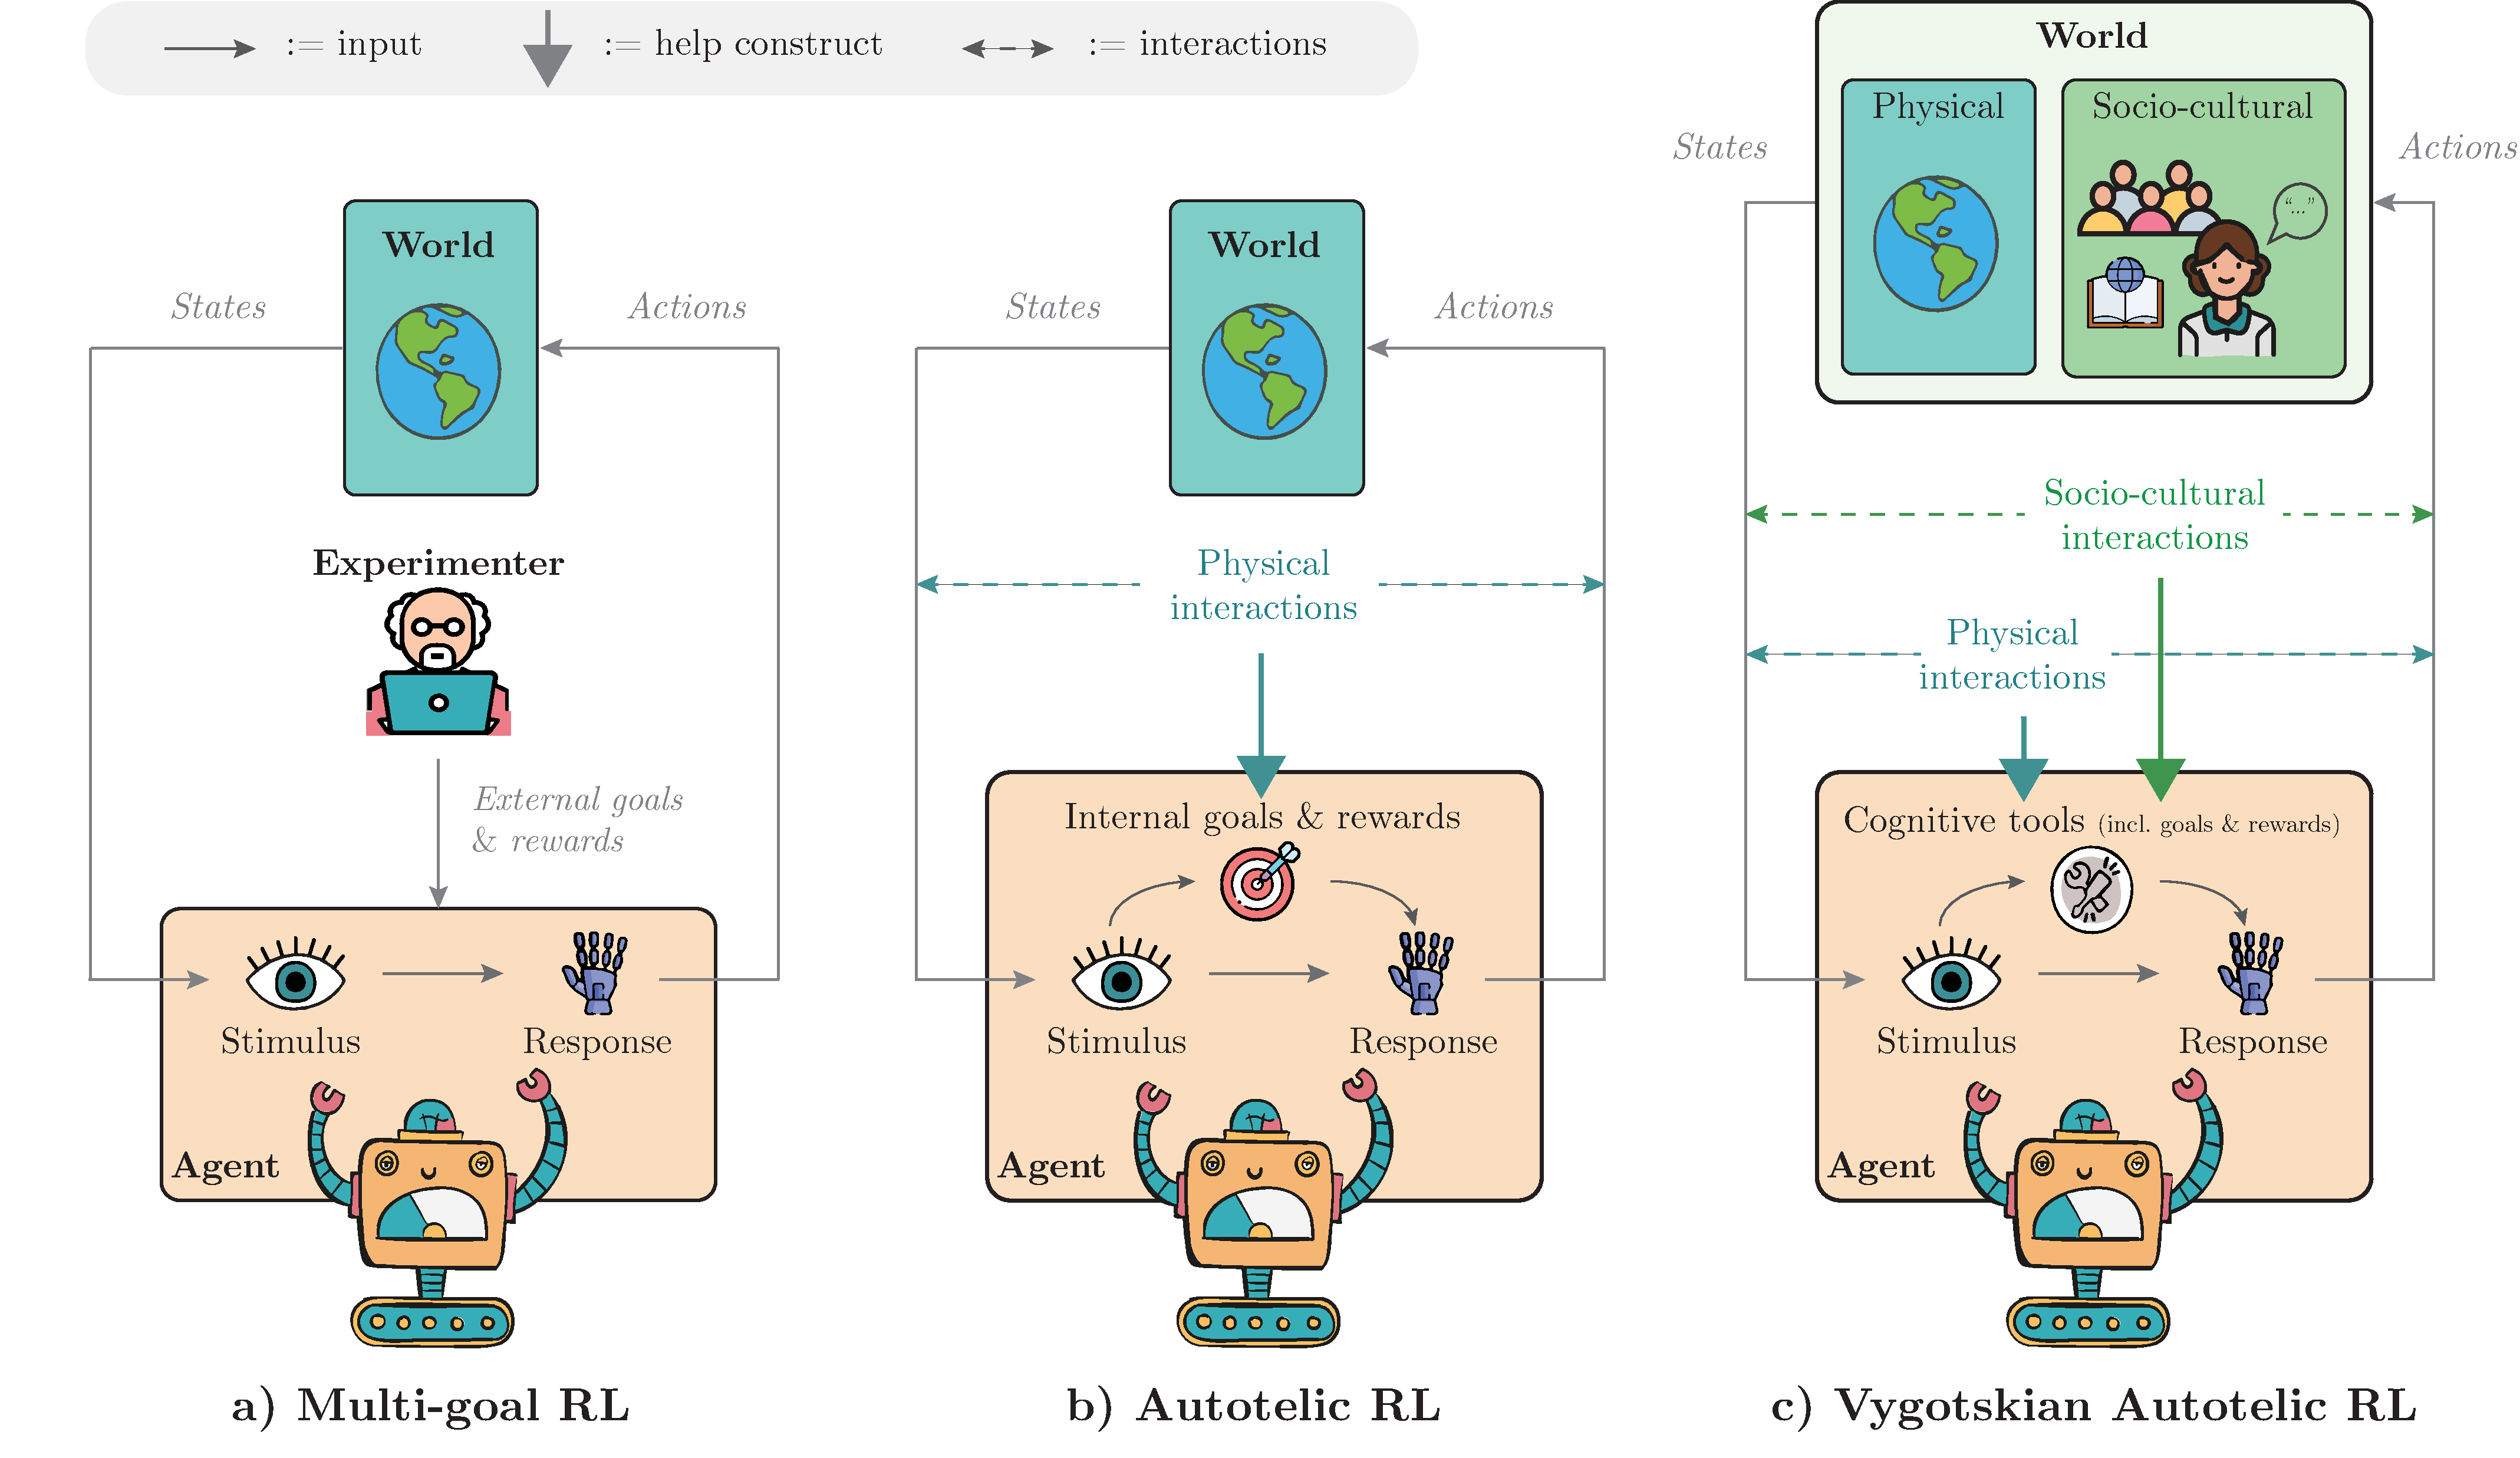
\includegraphics[width=\linewidth]{perspective/figure-intro-v4.pdf}
    \caption{\small From multi-goal RL to autotelic RL to Vygotskian autotelic RL. \rl defines an agent experiencing the state of the world as stimuli and acting on that world via actions. Multi-goal RL (a): goals and associated rewards come from pre-engineered functions and are perceived as sensory stimuli by the agent. Autotelic RL (b): agents build internal goal representations from interactions between their intrinsic motivations and their physical experience of the world (Piagetian view). Vygotskian autotelic RL (c): agents internalize physical and socio-cultural interactions into \textit{cognitive tools}. Here, \textit{cognitive tools} refer to any self-generated representation that mediates stimulus and actions. This can include self-generated goals, explanations, descriptions, attentional biases, visual aids, mnemotechnic tricks, etc. }
    \label{fig:rl_arl_varl}
\end{figure}

\vspace{.4cm}


% Piagetian view and autotelic learning
Jean Piaget, a pioneer of developmental psychology, demonstrated children's ability to set their own goals, shape their own learning trajectories, and develop in symbiosis with their physical environment.\cite{piaget1952origins} His work influenced future developments in both psychology and \ai.\cite{dautenhahn_studying_1999} Indeed, if each skill is the association of a goal (\eg ``be a good chess player'') and a policy to reach it, then \textit{open-ended skill discovery} presupposes the ability to invent and select one's own goals and reward functions so as to progressively build repertoires of skills. \textit{Autotelic \textsl{\rl}}\,---\,from the Greek \textit{auto} (self) and \textit{telos} (goal)\,---\,extends the \rl framework to build such agents.\cite{colas2021intrinsically} It integrates two extensions of the standard \rl framework: the ability to consider multiple goals in parallel (\textit{multi-goal \textsl{\rl}}) and the ability to represent and select one's own goals. Although the first extension is straightforward,\cite{schaul_universal_2015} the second requires another ingredient inspired by the study of human learning: \textit{intrinsic motivations}. 

% intrinsic motivations
Most of the human time is spent on activities that do not seem to satisfy any utilitarian end; think about children playing, or adults watching movies. Psychologists argue that such exploratory behaviors are powered by \textit{intrinsic motivations} (\im), a set of brain processes driving us to experience situations for the mere pleasure of experiencing novelty, surprise, or learning progress.\cite{berlyne_curiosity_1966,  kidd_psychology_2015, gottlieb_towards_2018}
Similar processes can be coded into artificial agents to foster spontaneous exploratory capabilities.\cite{schmidhuber_curious_1991, barto_intrinsic_2005, oudeyer_intrinsic_2007} Among them, \textit{knowledge-based \textsl{\im}} drive agents to experience parts of the environment to improve their internal models of the world and \textit{competence-based \textsl{\im}} let them improve their mastery of self-generated goals.\cite{oudeyer_what_2009} In the Piagetian tradition, autotelic agents see their goal representation and goal selection mechanisms emerge from interactions between competence-based \im and their experience of the physical world (see Figure~\ref{fig:rl_arl_varl}, b).\cite{colas2021intrinsically}

% limits of autotelic learning
In practice, current autotelic \rl implementations still lack human-like open-endedness. The goal representations emerging from their intrinsically motivated experience with the physical world end up very concrete and mostly consist in reaching target stimuli (\eg matching their visual input with a particular target).\cite{colas2021intrinsically} This contrasts with the wide diversity and the abstraction of goals targeted by humans. In addition, the generated goals very often belong to the distribution of previously experienced effects, which drastically limits the ability of autotelic agents to represent \textit{creative goals}, thus to explore and undergo an open-ended discovery process.\cite{colas_language_2020} Besides goal imagination, \rl algorithms still lack human-like capacities in terms of generalization, skill composition, abstraction, or sample efficiency.\cite{witty2021measuring,shanahan2022abstraction} 

% vygotsky and socio-cultural situatedness
The way forward might build on an alternative view of child development proposed by another pioneer of developmental psychology called Lev Vygotsky. Humans are social beings; intrinsically motivated to interact and cooperate with their peers.\cite{tomasello_cultural_1999,tomasello_understanding_2005, brewer2014addressing} For Vygotsky, linguistic social interactions such as descriptions, explanations, corrections, or play start as interpersonal processes before they are turned into \textit{intrapersonal} cognitive processes through the process of \textit{internalization}.\cite{vygotsky_thought_1934} Following his vision, many psychologists,\cite{berk_why_1994,lupyan_what_2012,gentner_analogy_2017} linguists,\cite{whorf_language_1956,rumelhart_sequential_1986,lakoff2008metaphors} and philosophers \cite{hesse1988cognitive,dennett_consciousness_1993,carruthers_magic_1998,carruthers_modularity_2002} argued for the importance of socio-cultural interactions in the development of human intelligence. 

What does this mean for \ai? We advocate for a \textit{Vygotskian Autotelic AI}. Specifically, we propose to immerse autotelic agents into our rich socio-cultural world; to let them interact with us and with their peers in natural language; to let them internalize these interactions and mesh them with their cognitive development (see Figure~\ref{fig:rl_arl_varl}, c). Just like they do for humans, language and culture will help shape the agents' goal representations and generation mechanisms, thereby offering them the ability to generate more diverse and abstract goals; to imagine new goals beyond their past experience. Because they will develop at our contact, bathed in our cultures, they will learn about our cultural norms, values, customs, interests, and thought processes; all of which would be impossible to learn in social isolation. Just like humans, machines will use language to develop higher cognitive functions like abstraction, generalization, or imagination.\cite{carruthers_language_1998, gentner_analogy_2017, dove_language_2018} As we will see, this process has already started. 

Recent advances in \ai make our proposition particularly timely. Indeed, these past years have seen a revolution in natural language processing (\nlp), the set of tools designed to analyze and generate language. Generative models of language trained on gigantic amounts of text can now produce high-quality language,\cite{brown2020language} handle multimodal inputs,\cite{radford2021learning,ramesh2022hierarchical,alayrac2022flamingo} and capture common sense\cite{west_symbolic_2021} or cultural artefacts.\cite{hershcovich_challenges_2022,arora2022probing} Pure language models like GPT-3\cite{brown2020language} are capable of impressive zero-shot generalizations including joke explanations, arithmetic, question answering, or even multi-step reasoning when nudged appropriately.\cite{creswell2022selection} Multi-modal variants can explain visual jokes (memes)\cite{alayrac2022flamingo} or generate impressive images from the most creative descriptions its testers can come up with.\cite{ramesh_zero-shot_2021,ramesh2022hierarchical} The ongoing convergence of autotelic \rl and \nlp will offer a wealth of opportunities as autotelic agents learn to interact with us, learn from us and teach us back. This motivates the elaboration of a theoretical framework to understand recent linguistic \rl developments and point towards future challenges in the quest for open-ended skill discovery.

This perspective extends previous calls to leverage Vygotsky's insights for a more socially-situated cognitive robotics.\cite{dautenhahn_studying_1999, zlatev_epigenesis_2001, lindblom_social_2003,mirolli_towards_2011} Zlatev discussed interactions between social-situatedness and epigenetic development,\cite{zlatev_epigenesis_2001} Dautenhahn and Billard drew the parallel between \ai and the Piagetian vs.\, Vygotskian views,\cite{dautenhahn_studying_1999} while Mirolli and Parisi, as well as Cangelosi et al., reviewed the first successful auxiliary uses of language for decision-making.\cite{mirolli_towards_2011, cangelosi2010integration} In the last decade however, the \ai community seems to have lost track of these insights. Today we update these arguments in the light of recent \ai advances and reframe the Vygotskian perspective within the autotelic \rl framework. As a result, we will not discuss non-embodied multi-modal supervised techniques\cite{radford2021learning, ramesh2022hierarchical, alayrac2022flamingo} or non-linguistic autotelic \rl.\cite{schaul_universal_2015} We will not cover the advances in the sub-field of \rl dedicated to the computational modeling of social interactions (social \rl).\cite{jaques2019social} Although future Vygotskian autotelic agents must incorporate social \rl mechanisms, current approaches do not consider autotelic agents able to set their own goals and, as such, do not tackle the open-ended skill discovery problem (see a complete discussion in a related paper\cite{sigaud_towards_2021}).

The next section sets the background and discusses the interaction between language and thought in humans by building on the work of psychologists and philosophers (Section~\ref{sec:4views}). The two following sections dive into the two key elements of a Vygotskian autotelic \ai identified in Section~\ref{sec:4views}: 1)~the ability to exploit information contained in linguistic structure and content (syntax, vocabulary, narratives) to support the development of cognitive functions (Section~\ref{sec:extraction}); 2)~the ability to internalize linguistic interactions within the agent to power its future autonomy and integration into the socio-cultural world (Section~\ref{sec:production}). Finally, Section~\ref{sec:challenges} identifies open challenges for future research.



% % % % % % % % % % % % % % % % % % % % % % % % % % % % % % % % % % % % % % % % % % % % 
% Section 1: Language and Thought in Humans
% % % % % % % % % % % % % % % % % % % % % % % % % % % % % % % % % % % % % % % % % % % % 
\subsection{Language and Thought in Humans, a Vygotskian Perspective}
\label{sec:language_and_though}
Our ability to generate new ideas is the source of our incredible success in the animal kingdom. But this ability did not appear with the first \textit{homo sapiens} 130,000 years ago. Indeed, the oldest imaginative artifacts such as figurative arts, elaborate burials or the first dwellings only date back to 70,000 years ago.\cite{harari_sapiens_2014, vyshedskiy_language_2019} This is thought to coincide with the apparition of \textit{recursive language}.\cite{goldberg1999emergence, vyshedskiy_language_2019, hoffmann_construction_2020} Which of these appeared first? Creativity or recursive language? Or did they mutually bootstrap?

Extreme views on the topic either characterize language as a pure communicative device to convey our inner thoughts (strong communicative thesis)\cite{chomsky_syntactic_1957,fodor1975language} or, on the other hand, argue that only language can be the vehicle of our thoughts (strong cognitive thesis)\cite{wittgenstein1953philosophical, mcdowell1996mind} As often, the truth seems to lie in between. Animal and preverbal infants demonstrate complex cognition,\cite{sperber1995causal, allen1999species} but language does impact the way we perceive,\cite{waxman_words_1995, yoshida_sound_2003} represent concepts,\cite{lakoff2008metaphors} conduct compositional and relational thinking,\cite{gentner2002relational, gentner_analogy_2017, vyshedskiy_language_2019} etc. Thus, language seems to be at least \textit{required} to develop some of our cognitive processes (requirement thesis), and might still be the vehicle of \textit{some} of our thoughts (constitutive thesis).\cite{carruthers_language_1998} Interested readers can find a thorough overview of this debate in \textit{Language and Thought} by Carruthers and Boucher.\cite{carruthers_language_1998}

If language is required to develop some of our higher cognitive functions, then autotelic artificial agents should use it as well. But how does that work? What is so special about language? 
Let us start with \textit{words}, which some called \textit{invitations to form categories}.\cite{waxman_words_1995} Hearing the same word in a variety of contexts invites humans to compare situations, find similarities, differences and build symbolic representations of agents, object and their attributes. With words, the continuous world can be simplified and structured into mental entities at various levels of abstraction. 

%The recursivity and partial compositionality of languages allow us to readily understand the meaning of sentences we never heard before by generalizing from known words and syntactic structures
The recursivity and partial compositionality of language allows us to readily understand the meaning of sentences we never heard before by generalizing from known words and syntactic structures. On the flip side, it also supports \textit{linguistic productivity},\cite{chomsky_syntactic_1957} the ability to generate new sentences\,---\,thus new ideas\,---\,in an open-ended way. 
Relational structures such as comparisons and metaphors facilitate our relational thinking,\cite{gentner2002relational, gentner_analogy_2017} condition our ability to compose mental images,\cite{vyshedskiy_language_2019} and support our understanding of abstract concepts such as emotions, politics or scientific theories.\cite{hesse1988cognitive,lakoff2008metaphors} 

Finally, language is a cultural artefact inherited from previous generations and shared with others. It supports our cultural evolution and allows humans to efficiently transfer knowledge and practices across people and generations\cite{henrich2003evolution,morgan_experimental_2015,chopra2019first}\,---\,a process known as the \textit{cultural rachet}.\cite{tomasello_cultural_1999} Through shared cultural artefacts such as narratives, we learn to share common values, customs and social norms, we learn how to navigate the world, what to attend to, how to think, what to expect from others.\cite{bruner1990acts} This cultural knowledge is readily accessible to children as they enter societies via social interactions and formal education. Learning language further extends the access to cultural artefacts such as books, movies, or the Internet. These act as a thousand virtual social partners to learn from. 

We now understand why language is so special. Let us focus on how it can shape cognitive development in humans and machines. Dennett, a proponent of the requirement thesis, suggests that linguistic exposition alone can lead to a fundamental cognitive reorganization of the human brain.\cite{dennett_consciousness_1993} He compares it to the installation of a serial virtual machine on humans' massively parallel processing brains. As a result, a slight change in our computational hardware (\eg compared to our primates relatives) could open the possibility for any cognitive software reprogramming driven by language, in turn triggering the learning and cultural evolution of higher cognitive capacities.
Carruthers, a proponent of the constitutive thesis, suggests that language may have evolved as a separate module to exchange inner representations with our peers (naive physics, theory of mind, etc). This would require connections between linguistic and non-linguistic modules to allow conversions between inner representations and linguistic inputs/outputs. In a similar way that humans can trigger imagined visual representations via top-down connections in their visual cortex, top-down activations of the linguistic module would create \textit{inner speech}. This hallucinated speech, when broadcast to other modules, would implement \textit{thinking in language}.\cite{carruthers1998thinking} Clark advances yet another possibility, the \textit{supra-communicative view}. Here, language does not transform the way the brain makes computations and is not the vehicle of thoughts. Instead, language complements our standard computation activities by ``\textit{re-shaping the computational spaces},'' turning problems that would be out of reach into problems our pattern-matching brains can solve.\cite{carruthers_magic_1998} In that sense, language is a \textit{cognitive tool} that enhances our cognitive abilities without altering them per se. 

Vygotsky's theory brings a complementary argument to this debate. Caretakers naturally scaffold the learning experiences of children, tailoring them to their current objectives and capacities. Through encouragement, attention guidance, explanations or plan suggestions, they provide cognitive aids to children in the form of interpersonal social processes.\cite{vygotsky_thought_1934} In this \textit{zone of proximal development}, as Vygotsky coined it, children can benefit from these social interactions to achieve more than they could alone. In these moments, children \textit{internalize} linguistic and social aids and progressively turn these interpersonal processes into intrapersonal \textit{psychological tools}.\cite{vygotsky_thought_1934}	 This essentially consists in building internal models of social partners such that learners can self-generate contextual guidance in the absence of an external one. Social speech is internalized into private speech (an outer speech of children for themselves), which, as it develops, becomes more goal-oriented and provides cognitive aids of the type caretakers would provide.\cite{vygotsky_thought_1934,berk_why_1994} Progressively, it becomes more efficient and abbreviated, less vocalized, until it is entirely internalized by the child and becomes \textit{inner speech}. 

This section showed why language is so important and might just be required for the development of our highest cognitive functions. If we want machines to show more human-like open-ended skill discovery processes, we might need to immerse them into rich socio-cultural worlds from the very beginning\,---\,just like we do with children\,---\,and equip them with tools to benefit from them. From the arguments above, we identify two key elements, see Figure~\ref{fig:extractive_productive}. First, we need autotelic agents to exploit the information contained within linguistic structures and contents. Exposed to language, agents will reorganize their internal representations for better abstraction, generalization and better alignment with human values, norms and customs (Dennett's thesis). Second, we need autotelic agents to internalize social interactive processes, \ie to \textit{model social partners within themselves} (Vygotsky's internalization). Social processes, turned into intrapersonal cognitive processes will orient the agent's focus, help it decompose tasks or imagine goals. This inner speech generation can serve as a common currency between other modules (\eg perception, motor control, goal generation) in line with Carruther's view and will help agent project problems onto linguistic spaces where they might be easier to solve (Clark's view). In the next two sections (\ref{sec:extraction}--\ref{sec:production}), we discuss these two key elements in detail and reframe recent works at the intersection of \rl and language in their light. 

\vspace{.4cm}
\begin{figure}[!ht]
    \centering
    \captionsetup{width=.85\linewidth}
    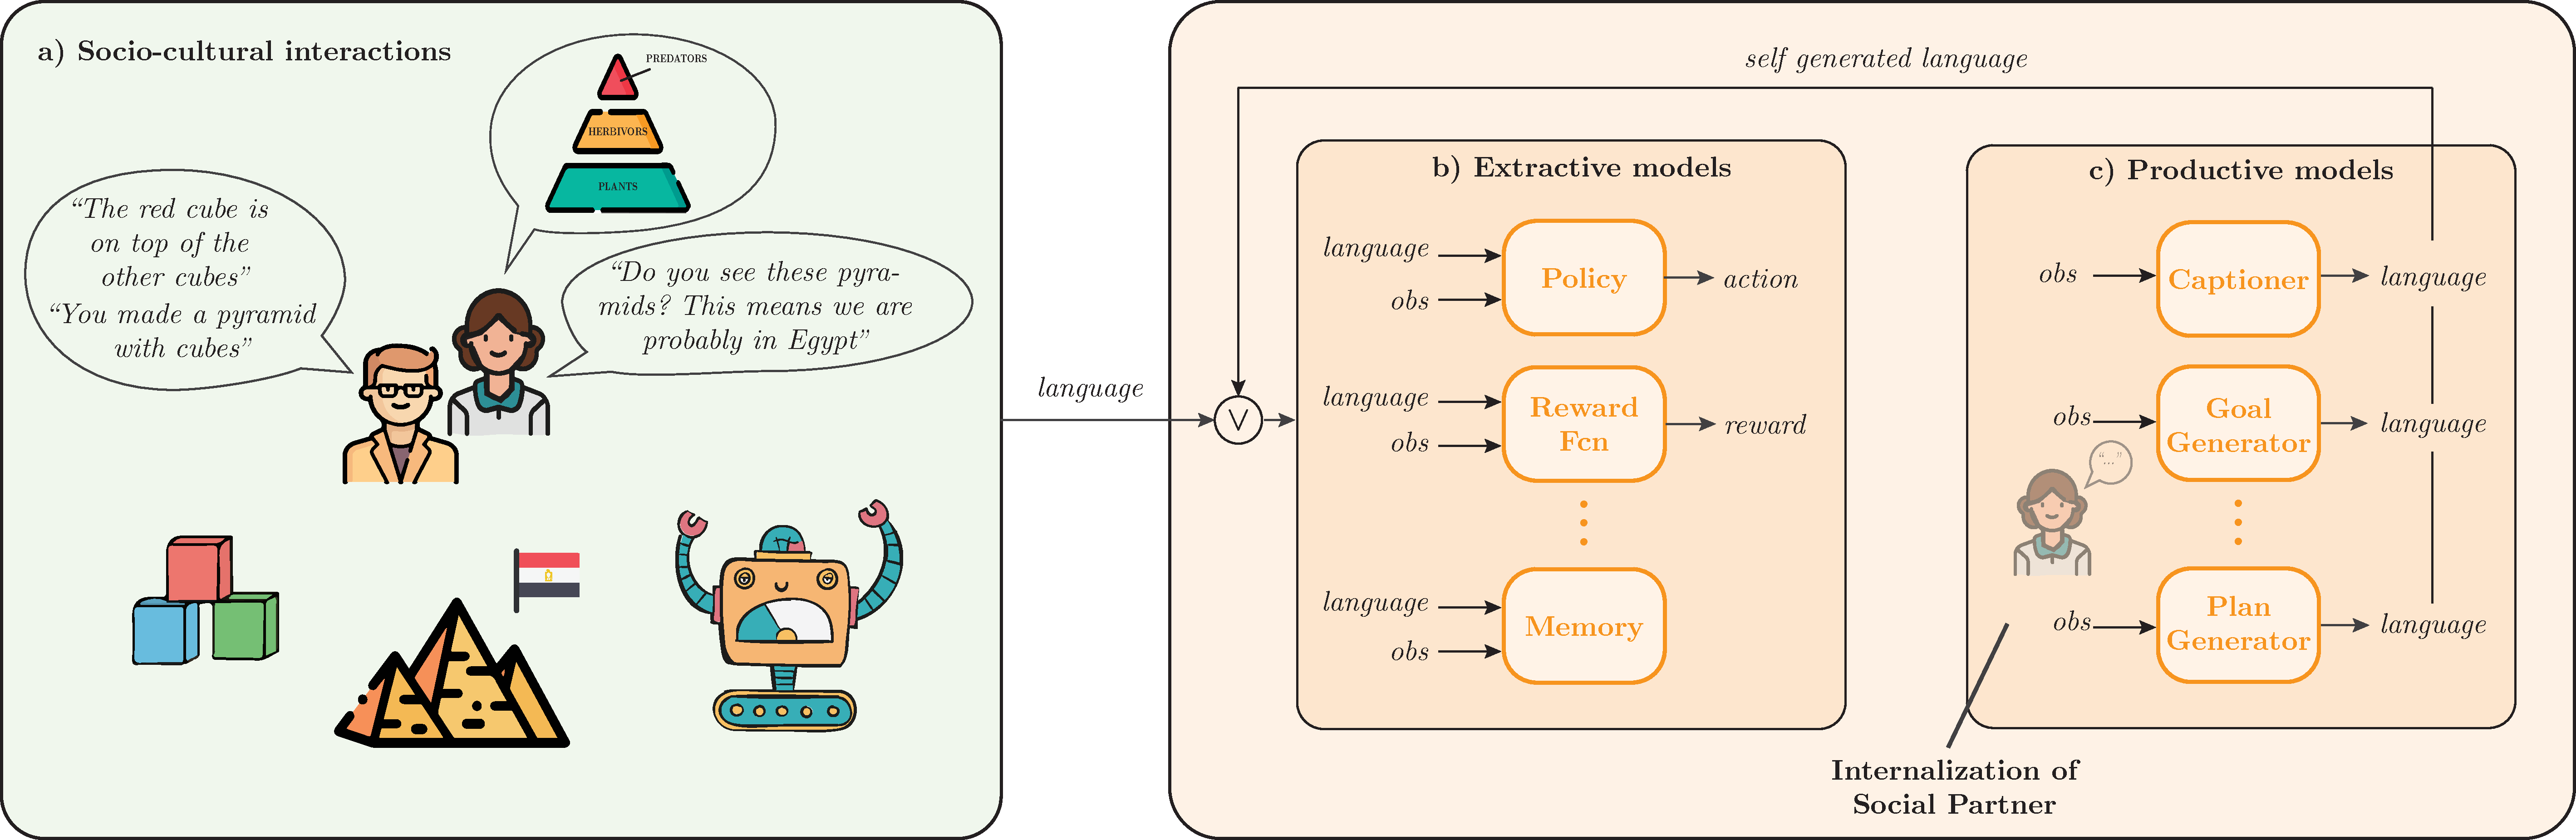
\includegraphics[width=1\linewidth]{perspective/extractive-productive-v3.pdf}
    \caption{\small The three components of Vygotskian autotelic agents: socio-cultural interactions, linguistic extraction and internalized linguistic production. Vygotskian autotelic agents are immersed into rich socio-cultural worlds where they experience a variety of linguistic feedback including descriptions, explanations, or metaphors (a). They can exploit information from linguistic structures and content by conditioning their internal modules on this feedback (b, extractive models). Finally, they learn to internalize social interactions by training productive models of language to generate feedback similar to the one they receive from others (c, productive models). This offers agents the autonomy to build their own cognitive tools, bootstrapped by socio-cultural language.}
    \label{fig:extractive_productive}
\end{figure}
\vspace{.4cm}


% % % % % % % % % % % % % % % % % % % % % % % % % % % % % % % % % % % % % % % % % % % % 
% Section: Extraction of Regularities from Language
% % % % % % % % % % % % % % % % % % % % % % % % % % % % % % % % % % % % % % % % % % % % 
\subsection{Exploiting Linguistic Structure and Content}
\label{sec:extraction}

In its vocabulary, syntax and narratives, language offers both powerful computational tools for thinking and important cultural knowledge about the world. According to Dennett's thesis, mere exposure to language can already help agents rewire their inner processes and develop new abilities. Recent advances in \ai seem to support that idea.

\textbf{Learning to abstract and generalize.} Exposition to linguistic labels is known to facilitate category learning in humans,\cite{waxman_words_1995, yoshida_sound_2003} but also in machines.\cite{lupyan_carving_2005} As Mirolli and Parisi defend, the repeated occurrence of a linguistic label (\textit{red} in their example) leads to the conflation of internal representations associated with that label (red things) which, in turn, facilitates further classifications based on the linguistic attributes.\cite{mirolli_towards_2011}

We see a similar effect in \rl agents targeting linguistic goals. The exposure to aligned instructions and trajectories seems to reshape the internal representations of the agent contained within its action policy. The policy is a neural network-based function conditioned on the agent's instruction that maps the current state of the world to its next actions. By \textit{internal representations}, we mean representations computed within the layers of the policy to facilitate the final decision-making. When repeatedly asked to grasp \textit{red objects}, the policy learns to focus on objects' colors to facilitate action selection.\cite{hill_emergent_2019,colas_language_2020} \textit{Red} is an abstraction over a continuous space of colors. It is first cultural, outside of the agent, but gets progressively internalized within the agent via a combination of linguistic exposure and decision-making. 

Exposed to a diversity of instructions, agents gain new cognitive abilities. The first is \textit{abstraction}. Linguistic autotelic agents can reach and make sense of abstract  relational goals ``\textit{sort objects by size},''\cite{jiang_language_2019} ``\textit{put the cylinder in the drawer},''\cite{lynch_grounding_2020} sequential goals ``\textit{open the yellow door after opening a red door},''\cite{chevalier-boisvert_baby-ai_2019} or even learning goals ``\textit{is the ghargh edible?}.''\cite{yuan_interactive_2019} Whereas handling abstract goals used to require engineers to hard-code specific goal representations and reward functions within the agent,\cite{curious,team2021open} linguistic goals offer abstraction via simple linguistic interactions.\cite{bahdanau_learning_2019,colas_language_2020} Once abstractions have been distilled within the representations of the agent, they can be leveraged to augment its exploratory capacities. Searching for novelty in a space of abstract linguistic descriptions of the world is indeed more efficient than searching for novelty in low-level sensorimotor spaces which could be trivially triggered by leaves moving in the wind or TV noise.\cite{tam2022semantic, Mu2022ImprovingIE}

A second cognitive ability is \textit{systematic generalization}. Language-instructed agents indeed seem to demonstrate the ability to generalize to new instructions obtained by systematic recombinations of instructions they were trained on.\cite{hill_emergent_2019} For instance, agents that learned to \textit{grasp blue objects} and \textit{put green objects on the table} can directly \textit{grasp green objects} and \textit{put blue objects on the table}.\cite{Hermann2017, chevalier-boisvert_baby-ai_2019, bahdanau_learning_2019, hill_emergent_2019, hill_human_2020, colas_language_2020, sharma2021skill, karch2021grounding} This ability can either be encoded in learning architecture through the use of modular networks (neuro-symbolic approaches), or emerge spontaneously in plain networks under the right environmental conditions.\cite{hill_emergent_2019} Although sometimes the world does not conform to strict linguistic compositionality, systematic generalization still supports good priors\,---\,\eg \textit{feeding the cat} is not a strict transposition of \textit{feeding the plant} but they still share similarities (bringing supplies to the cat/plant).\cite{colas_language_2020}

\textbf{Learning to represent possible futures.} After being exposed to aligned trajectories and linguistic descriptions, agents can generate concrete examples of abstract descriptions. The \decstr approach, for example, trains a generative world model to sample from the distribution of possible future states matching a given abstract linguistic description.\cite{akakzia_grounding_2021} This simple mapping supports \textit{behavioral diversity}, the ability to represent different possible futures so as to select one to pursue. Similar setups could leverage \dalle, an impressive text-to-image generative system.\cite{ramesh_zero-shot_2021,ramesh2022hierarchical} Trained on pairs of images and compositional descriptions, \dalle can generate high-quality images from the most twisted descriptions humans can think of. The exposition to compositional language, paired with sufficiently powerful learning architectures and algorithms leads to impressive visual composition abilities that could be put to use to generate visual goals or to represent possible futures in embodied and situated agents. 

\textbf{Learning to decompose tasks.} Vygotsky and others discovered that children's use of private speech helps them increase self-control and is instrumental to their capacity to reason and solve hard tasks.\cite{vygotsky_thought_1934, berk_why_1994} The ability to formulate sentences like ``at the left of the blue wall,'' for instance, predicts spatial orientation capacities in such contexts, while interfering with adult's inner speech via speaking tasks hinders theirs.\cite{hermer-vazquez_language_2001}

Language indeed contains cues about how to decompose tasks into sub-tasks, \ie how to \textit{generate good plans}. Although \textit{gharble} is a made-up word, \textit{fry the gharble} probably involves a preparation of the gharble (\eg peeling, cutting), some sort of oil and a frying pan.\cite{yuan_interactive_2019} \textit{Draw an octogon} contains cues about the decomposition of the task: \textit{octo} means 8, so we should probably do something 8 times, etc.\cite{wong_leveraging_2021} Recent \ai approaches leverage these regularities by training \textit{plan generators} from linguistic task descriptions.\cite{jiang_language_2019, chen_ask_2021, sharma2021skill, mirchandani2021ella, shridhar_alfworld_2021, wong_leveraging_2021} Among them, Wong et al.\, use plan generation as an auxiliary task to train a drawing policy.\cite{wong_leveraging_2021} Generating plans to solve a particular drawing task helps shape the internal representation of the main policy which, they find, favors abstraction and generalization in the main task. Interestingly, language only shapes representations and is not required at test time, in line with the requirement thesis of Dennett.

Inspired by video games of the 80s such as \textit{Zork}, text-based environments define purely linguistic goals, actions and states.\cite{cote_textworld_2018, das_embodied_2018, yuan_interactive_2019} Training a policy in such environments can be seen as training a plan generator in a linguistic world model, \ie training an inner speech to generate good task decompositions. This idea was exploited in \textit{AlfWorld}, where a pre-trained plan generator is deployed in a physical environment to generate sub-goals for a low-level policy.\cite{shridhar_alfworld_2021} Here, the abstraction capabilities of language help the plan generator solve long-horizon tasks.

The above approaches echo the thesis of Dennett (Section~\ref{sec:4views}): the mere exposure to structured language, once internalized within internal modules (reward function, policy, world model) strongly shapes inner representations in new ways and supports new cognitive functions (abstraction, future states generation, compositional generalization, task decomposition, etc).

 %Other methods take a complementary approach: they train advice-conditioned low-level policies and distill them into high-level task policies via supervised learning.\cite{watkins2021teachable}
\textbf{Learning from cultural artefacts.} Large language models (\llm) are trained on huge quantities of text scrapped from the internet: Wikipedia, forums, blogs, scientific articles, books, subtitles, etc.\cite{devlin2019bert,brown2020language} As such, they can be seen as \textit{cultural models} that contain information about our values, norms, customs, history, or interests.\cite{hershcovich_challenges_2022,arora2022probing} This represents a great opportunity for autotelic agents to learn about us, align with us, and better navigate our complex world. So far, only very little research has leveraged that opportunity. An example is the use of a trained \llm to act as a zero-shot planner, \ie a plan generator.\cite{huang2022language} Plugged with an interactive agent, the language model is used to generate sub-goals for the agent to solve the main task. Another work extracts information about complex time-extended behaviors from an \llm by asking it to score the actions available to the agent.\cite{ahn2022doasican}. Finally, the MineDojo framework\cite{fan2022minedojo} proposes to caption thousands of YouTube videos of humans playing Minecraft using GPT-3\cite{brown2020language}, generating creative high-level tasks as well as low-level linguistic guidance for embodied agents. Challenge~\#3 of Section~\ref{sec:challenges}  discusses more opportunities to harness these cultural models for open-ended skill discovery. 

% % % % % % % % % % % % % % % % % % % % % % % % % % % % % % % % % % % % % % % % % % % % 
% Section : Internalization of Language Production
% % % % % % % % % % % % % % % % % % % % % % % % % % % % % % % % % % % % % % % % % % % % 
\subsection{Internalization of Language Production}
\label{sec:production}

Agents that internalize extractive models learn to exploit the information contained within linguistic vocabularies, structures and narratives. However, most of them require external linguistic inputs at test time and, thus, cannot be considered autonomous. Vygotskian autotelic agents reach autonomy by internalizing \textit{productive models}; \ie by learning to generate their own linguistic inputs, their own \textit{inner speech} (see Figure~\ref{fig:extractive_productive}, c). 

Inner speech can be understood as a fully-formed language: descriptions, explanations or advice to be fed back to extractive models; to serve as a common currency between cognitive modules (fully-formed inner speech).\cite{zeng2022socratic} But it might also be understood as \textit{distributed representations} within productive models, \textit{upstream from fully-formed language} (distributed inner speech). In the latter interpretation, linguistic production acts as an auxiliary task whose true purpose is to shape the agent's cognitive representations. Symbolic behaviors might indeed not require explicit symbolic representations but may emerge from distributed architectures trained on structured tasks, \eg involving linguistic predictions.\cite{mcclelland2010letting,santoro2021symbolic} 
In the literature, we found four types of productive models making use of either fully-formed or distributed inner speech: trajectory captioners, plan generators, explanation generators and goal generators. 

\textbf{Trajectory captioners.} Trajectory captioners are trained on instructive or descriptive feedback to generate valid descriptions of scenes or trajectories.\cite{cideron_higher_2020, zhou_inverse_2020, colas_language_2020, nguyen2021interactive, yan2022intra} In line with Vygotsky's theory, these agents internalize models of descriptive social partners. They generate an \textit{inner speech} describing their ongoing behaviors just like a caretaker would. Used as an auxiliary task (distributed inner speech), the generation of descriptions helps the agent shape its representation so as to generalize better to new tasks.\cite{yan2022intra} With fully-formed inner speech, agents can generate new multi-modal data autonomously, and learn from past experience via \textit{hindsight learning},\cite{andrychowicz_hindsight_2017} \ie the reinterpretation of their trajectory as a valid behavior to achieve the trajectory's description.\cite{zhou_inverse_2020, colas_language_2020, nguyen2021interactive}

\textbf{Plan generators.} Plan generators are both extractive and productive. Following the formalism of hierarchical \rl (\hrl), plan generators are implemented by a \textit{high-level policy} generating linguistic sub-goals to a low-level policy (executioner).\cite{dayan_feudal_1993, sutton_between_1999} Linguistic sub-goals are a form of inner speech that facilitates decision-making at lower temporal resolution by providing abstract, human-interpretable actions, which themselves favor systematic generalization for the low-level policy (see Section~\ref{sec:extraction}).\cite{jiang_language_2019, chen_ask_2021, shridhar_alfworld_2021} Here, agents internalize linguistic production to autonomously generate further guidance for themselves in fully-formed language (task decompositions). 

\textbf{Explanation generators.} Vygotskian agents can generate \textit{explanations}. Using the generation of explanations as an auxiliary task (distributed inner speech) was indeed shown to support causal and relational learning in complex \textit{odd one out} tasks.\cite{lampinen_tell_2021} Note however that this approach is neither embodied, nor autotelic.

\textbf{Goal generators.} Some forms of creativity appear easier in linguistic spaces because swapping words, compositing new sentences, and generating metaphors are all easier in the language space than in sensorimotor spaces. The \imagine approach leverages this idea to support \textit{creative goal imagination}.\cite{colas_language_2020} While previous methods were limited to generating goals within the distribution of past experience (\eg with generative models of states\cite{nair2018visual}), \imagine invents out-of-distribution goals by combining descriptions of past goals. These manipulations occur in linguistic spaces directly and are thus \textit{linguistic thoughts}; fully-formed inner speech (Carruthers' view). The problem of goal imagination, difficult to solve in sensorimotor space, is projected onto the linguistic space, solved there, and projected back to sensorimotor space (Clark's view). This, in turn, powers additional cognitive abilities. First, it powers a creative exploration oriented towards objects and interactions with them. Second, it enhances systematic generalization by widening the set of goals the agent can train on.\cite{colas_language_2020}

By internalizing linguistic production, \imagine generates goals that are both \textit{novel} (new sentences) and \textit{appropriate} (they respect linguistic regularities, both structures, and contents).\cite{runco_standard_2012} Social descriptions focus on objects, object attributes, and interactions with these objects. Imagined goals obtained by recompositions of social ones share the same attentional and conceptual biases, \eg by reusing semantic categories of a particular culture. Thus, cultural biases are implicitly transmitted to the agent, which forms goal representations and biases goal selection following cultural constraints.\cite{colas_language_2020}

Note that productive models are very rare in the literature. In the future, Vygotskian autotelic agents must learn to internalize productive models for all types of multi-modal feedback they encounter: advice, explanations, attention guidance, motivation, instructions, descriptions, etc. It is only by learning to generate this guidance for themselves that they may gain full control of their own behavior. The question of whether to use fully-formed or distributed inner speech remains open, as both strategies seem to find different use-cases. Because cultural models are biased, future agents will need to edit, correct, augment and generate their own interpretations of culture based on their individual experiences. How to efficiently steer language models in these ways remains a question to explore in future research. 

%
%% % % % % % % % % % % % % % % % % % % % % % % % % % % % % % % % % % % % % % % % % % % % 
%% Section : Discussion
%% % % % % % % % % % % % % % % % % % % % % % % % % % % % % % % % % % % % % % % % % % % % 
%\subsection*{Conclusion}
%% The Discussion should be succinct and must not contain subheadings.
%
%This perspective builds on the autotelic \rl framework inspired by the Piagetian tradition to propose a complementary view motivated by Vygotsky's work: a \textit{Vygotskyan Autotelic AI}. Recent works at the intersection of deep \rl and \nlp present promising first steps, but a lot remains to be done. Vygotskian autotelic agents will interact with us and with our culture, exploit linguistic structures and content and finally internalize social interactions to serve as the basis of their future cognitive functions: abstraction, compositional thinking, generalization or imagination. 
%
%Vygotskian Autotelic \ai opens a new research program with exciting opportunities. The current \nlp revolution can be harnessed to design more interactive and teachable agents. As they interact with humans and their peers in rich socio-cultural worlds, they will learn to leverage cultural and linguistic knowledge to bootstrap their cognitive development, and may eventually contribute back to our shared cultural evolution. This perspective uncovers an important challenge: how will we train and leverage cultural models to align with the values of human cultures so as to educate ethical and useful artificial agents?
%
%Dennett used the software/hardware metaphor to describe the impact of language on human brains.\cite{dennett_consciousness_1993} Current \ai research mostly focuses on \textit{hardware} by asking \textit{how can we design better learning architectures and algorithms?} In complement, this paper suggests to focus on \textit{software} as well: \textit{How can we build the right socio-cultural bath which, combined with efficient hardware, will allow the emergence of a more human-like \ai}?
%
%
%
